\subsection{Deriving group sequential designs using boundary families  \label{sec:boundfam}}
The second method of setting boundaries uses the relative $z$-value for a design cutoff at each interim analysis, $c_i>0$, $i=1,2,\ldots,k$.
We define vectors ${\bf t}\equiv (t_1,t_2,\ldots,t_k)$ and ${\bf c}\equiv (c_1,c_2,\ldots,c_k)$.
For 2-sided testing, Wang and Tsiatis \cite{WangTsiatis} defined the boundary function 
\begin{equation}
-a_i=b_i=C({\bf t},{\bf c})c_i
\end{equation}
where the constant $C({\bf t},{\bf c})>0$ is chosen to appropriately control Type I error. 

Wang and Tsiatis \cite{WangTsiatis} specifically defined the boundary function family
\begin{equation}
g(t;\Delta)=C({\bf t}; \Delta)t^{\Delta-.5}.
\end{equation}
For $i=1,2,\ldots,k$ the boundary at analysis $i$ are given by
\[
-a_i=b_i=C({\bf t}; \Delta)t_i^{\Delta-.5}.
\]
For 2-sided testing, note that for $\Delta=.5$ the boundary values are all equal. Thus, this is equivalent to a Pocock \cite{PocockBound} boundary when analyses are equally spaced.
The value $\Delta=0$ generates O'Brien-Fleming bounds \cite{OF}. 

Pampalona and Tsiastis \cite{PampallonaTsiatis} derived a related method of using boundary families to set asymmetric bounds; this is not currently implemented in \texttt{gsDesign()}. 
Using constants $c^\prime_i>0$, $i=1,2,\ldots,k$ and a constant $C^\prime(\bf t; I_k)$ that along with $I_k$ is used to appropriately control Type II error, they set
\begin{equation}
a_i=\delta\sqrt{t_i}-C^\prime({\bf t})c_i^\prime.
\end{equation}

O'Brien-Fleming, Pocock, or Wang-Tsiatis are normally used with equally-spaced
analyses. 
They are used only with one-sided (\texttt{test.type=1}) and symmetric two-sided (\texttt{test.type=2}) designs.
We will use the CAPTURE example, again with 80\% power rather than the default of 90\%. 
Notice that this requires specifying \texttt{beta=.2} in both \texttt{nBinomial()} and \texttt{gsDesign()}.
O'Brien-Fleming, Pocock, or Wang-Tsiatis (parameter of 0.15) bounds for equally space analyses are generated using the parameters \texttt{sfu} and \texttt{sfupar} below. If you print the Pocock design (\texttt{xPocock}), you will see that the upper bounds are all equal and that the upper boundary crossing values  $\alpha_i(0)$ printed in the \texttt{Spend} column decrease from .0091 for the first analysis to .0041 for the final analysis.

\bigskip

\begin{verbatim}
n.fix <- nBinomial(p1=.15, p2=.1, beta=.2)
xOF <- gsDesign(k=4, test.type=2, n.fix=n.fix, sfu="OF", beta=.2)
xPocock <- gsDesign(k=4, test.type=2, n.fix=n.fix, sfu="Pocock", beta=.2)
xWT <- gsDesign(k=4, test.type=2, n.fix=n.fix, sfu="WT", sfupar=.15, beta=.2)
\end{verbatim}
The resulting sample sizes for these designs can be computed using
\begin{verbatim}
nOF <- 2 * ceiling(xOF$n.I[4] / 2)
nPocock <- 2 * ceiling(xPocock$n.I[4] / 2)
nWT <- 2 * ceiling(xWT$n.I[4] / 2)
\end{verbatim}
We now present an example of how is fairly simple to produce custom plots using \texttt{gsDesign()} output and standard R plotting functions. The resulting output is in Figure \ref{fig:WT}. If you are not familiar with R plotting, executing the following statements one at a time may be instructive.
The call \texttt{help(plot)} and its "See also" links (especially \texttt{par}) can be used to find explanations of parameters below.
The \texttt{legend} call below particularly demonstrates a nice strength of R for printing greek characters and subscripts in plots.
\begin{verbatim}
plot(xOF$n.I,xOF$upper$bound,xlim=c(300,1800),ylim=c(1.5,4.5),cex=1.5,lwd=2,
     type="b",xlab="N",ylab="Normal critical value (upper bounds)",pch="o",
     main="N and upper bounds with Wang-Tsiatis designs")
lines(xPocock$n.I,xPocock$upper$bound,lty=3,lwd=2)
points(xPocock$n.I,xPocock$upper$bound,pch="p",cex=1.5)
lines(xWT$n.I,xWT$upper$bound,lty=2,lwd=2)
points(xWT$n.I,xWT$upper$bound,pch="x",cex=1.5)
legend(x=c(750,1825), y = c(3.7,4.5), lty=c(1,2,3), lwd=2, pch=c("o","x","p"),
       cex=1.5,
       legend=c(expression(paste(Delta,"=0.0, ",N[4],
                "=1404, (O'Brien-Fleming)")), 
       c(expression(paste(Delta,"=.15, ",N[4],"=1430")), 
       c(expression(paste(Delta,"=.50, ",N[4],"=1650, (Pocock)"))))))
\end{verbatim}

\bigskip
\begin{figure}
\begin{center}
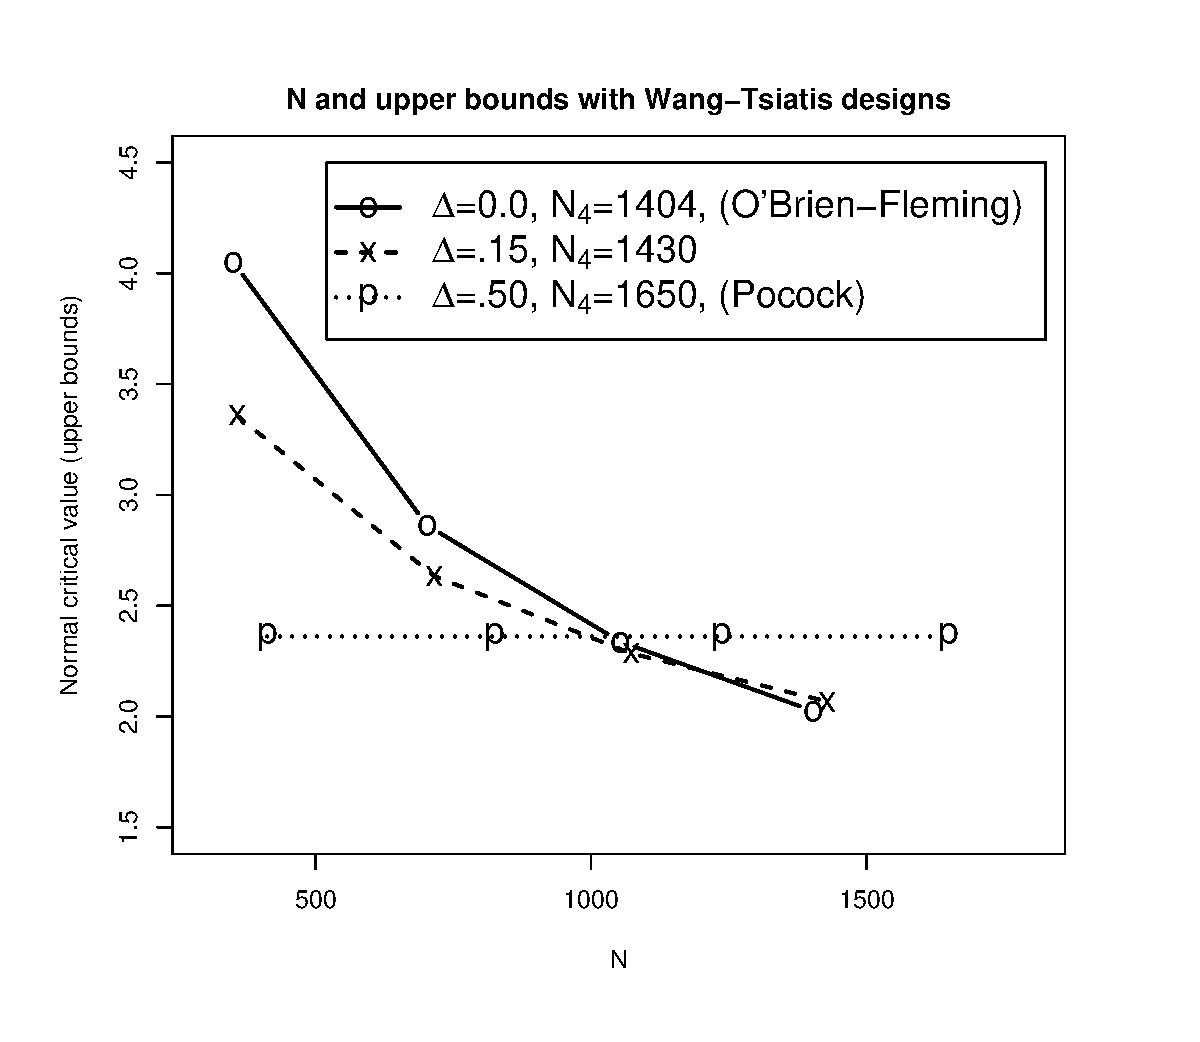
\includegraphics[width=.6\textwidth]{figs/WTCAPTURE.pdf}
\end{center}
\caption{Wang-Tsiatis bounds for the CAPTURE example\label{fig:WT}}
\end{figure}%

Figure \ref{fig:WT} shows how the upper bounds and sample size change as $\Delta$ changes for Wang-Tsiatis bounds. 
For the O'Brien-Fleming design, the final sample size is only inflated to 1402 from the 1372 required for a fixed design.
The relatively aggressive early bounds for the the Pocock design result in sample size inflation to 1650. 
This design is not frequently used because of the relatively low bounds at early analyses and the substantial sample size inflation required to maintain the desired power. 
Since the nominal p-value required for stopping at the initial analysis for the O'Brien-Fleming design is .00005 (2-sided), an intermediate design with $\Delta=.15$ might be of some interest. 
This has a relatively small sample size inflation to 1430 in order to maintain power and the nominal p-value required to stop the trial at the first interim analysis is .0008 (2-sided).   
Examine the boundary crossing probabilities by reviewing, for example,
\texttt{xOF\$upper\$spend}.
Also consider reviewing \texttt{plot(xWT, plottype=3)} to see the observed treatment effect required at each analysis to cross a boundary.
